\section{Alloy results}
 These are the results of the model.
\begin{figure}[h!]
	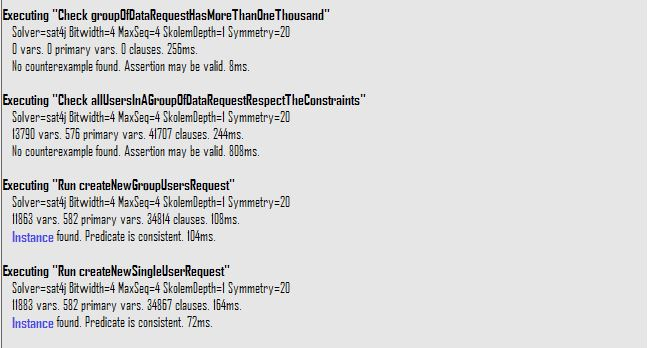
\includegraphics[width=1.00\textwidth]{./pictures/alloy_execute1.JPG}
\end{figure}
\begin{figure}[h!]
	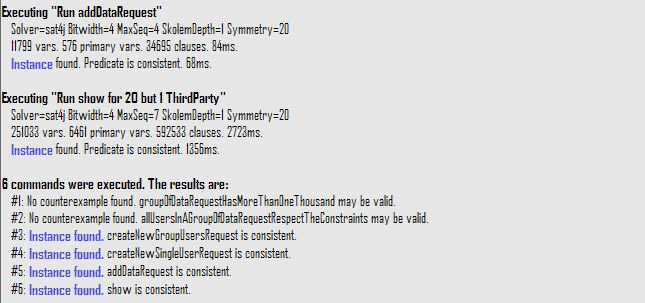
\includegraphics[width=1.00\textwidth]{./pictures/alloy_execute2.JPG}\par
	\caption{Results of check and run commands}
\end{figure}

\section{Alloy worlds}
In this section there are three different examples of worlds descibed by the model:
\begin{itemize}
	\item figure 4.2 highlights the metamodel related to the code written above;
	\item figure 4.3 provides a sample of a third party with an accepted GroupUsersRequest and a refused one. To obtain an 			accepted GroupUsersRequest the bound of 1000 has been reduced to 2; 
	\item figure 4.4 has the aim to show how the model behaves with a SingleUserRequest.
	
\end{itemize}

\begin{figure}[h!]
	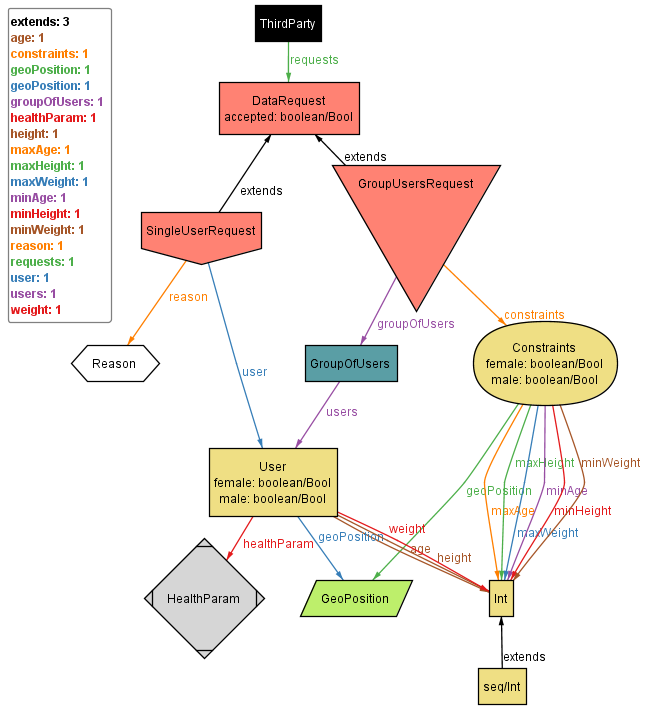
\includegraphics[width=1.00\textwidth]{./pictures/world3.png}\par
	\caption{This figure represent the metamodel of the code written above}
\end{figure}

\begin{figure}[h!]
	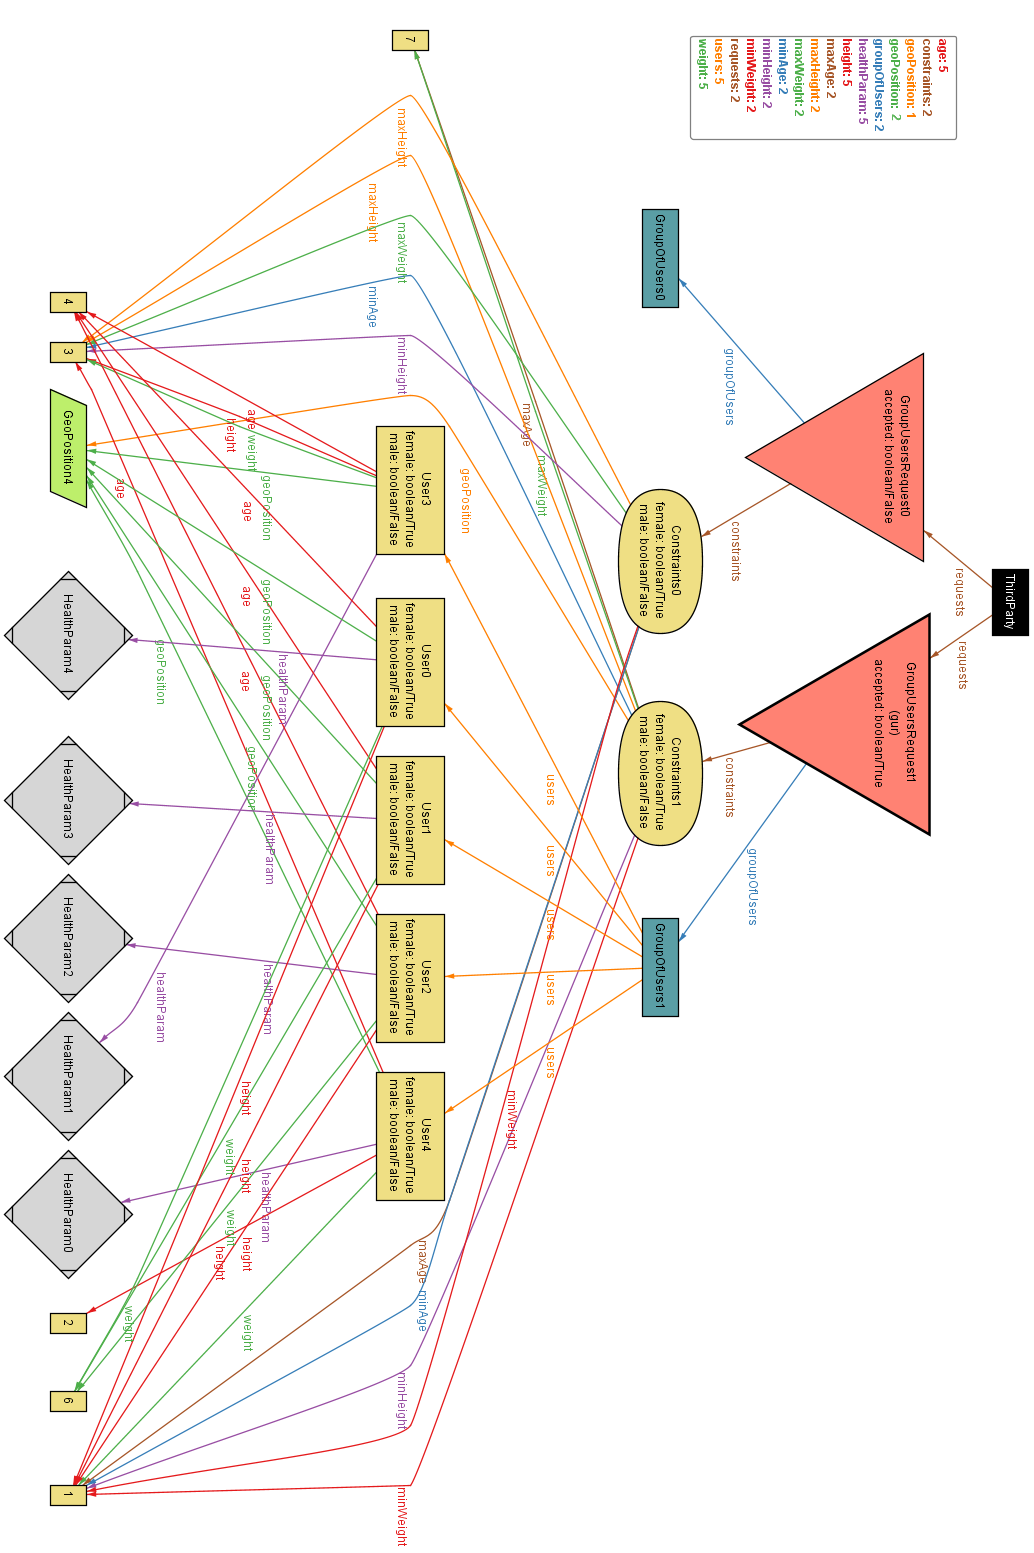
\includegraphics[width=1.00\textwidth]{./pictures/world2.png}\par
	\caption{This figure represent a third party with two GroupUsersRequest}
\end{figure}

\begin{figure}[h!]
	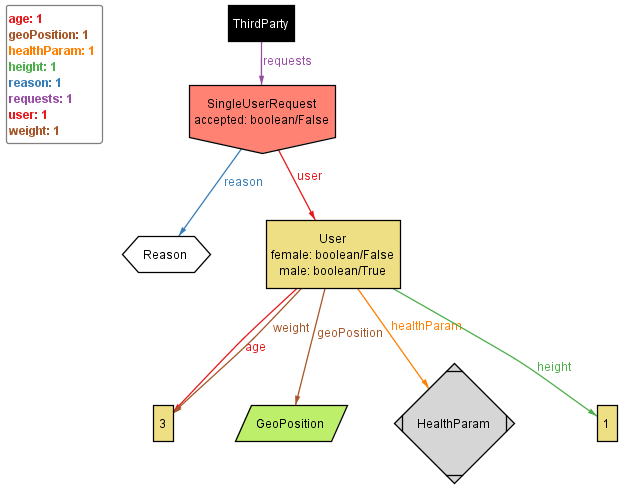
\includegraphics[width=1.00\textwidth]{./pictures/world1.png}\par
	\caption{This figure represent a third party with a SIngleUSerRequest}
\end{figure}